\documentclass[12pt, letterpaper]{article}
\usepackage[utf8]{inputenc}
\usepackage{amsmath}
\usepackage{graphicx}
\usepackage{fullpage}

\title{Generating Traffic Matrices}
\date{}
 
\begin{document}

\maketitle

Here we describe how traffic matrices are generated by
\verb|tm-gen|. As a starting point we used the gravity-based model
from~\cite{tm-synthesis-ccr05}, which we briefly rehash here. In that
model the volume of traffic ($T(n_i,n_j)$) for each of the $N(N-1)$
pairs in the network is obtained by:

\begin{equation}
\label{eq:tm-gen}
T(n_i,n_j) = T \frac{T^{in}(n_i)}{\sum_{k} T^{in}(n_k)} \frac{T^{out}(n_j)}{\sum_{k} T^{out}(n_k)}
\end{equation}

where $T$ is the total traffic in the network. The values
$T^{in}(n_i)$ and $T^{out}(n_i)$ are drawn from an exponential
distribution. This model has been shown to produce realistic traffic
matrices, even though it uses only a single parameter---the mean value
of the exponential distribution. While it represents a good starting
point, we note that this simple approach exhibits a couple of
significant drawbacks.

The first one is that there are no guarantees that the network will be
able to fit the resulting traffic matrix. The level of saturation of
the network depends on both the mean value of the exponential and the
actual network topology. On one hand it may be that we pick a mean
value that results in a traffic matrix that exceeds the maximum flow
of the network---{\em i.e.,} one for which no routing scheme will ever be
able to fit the demand. On the other hand, if we pick a mean value
which is too low we will generate a traffic matrix that is
trivial---{\em i.e.,} one for which every aggregate can be completely
routed on its shortest path without causing congestion.

Ideally we would like to have better control over the network's load
level. We take the approach of previous work~\cite{haddadi2013recent}, which suggests
scaling the traffic matrix after generation in order to set the
network's load to an arbitrary point between the two extremes
described above. To do so we first generate a traffic matrix using a random
exponential distribution with an arbitrary mean value. We then obtain
the minimum maximal link utilization possible under any routing scheme
by solving the theoretically optimal MinMax multi-commodity flow
problem (e.g., as described here~\cite{TeXCP-Kandula05}). If this link
utilization value is $u$, then we know that network is $1/u$ away from
being saturated---{\em e.g.,} if $u=0.3$ then we know that if we scale
all demands by $1 / 0.3 = 3.3$ we will achieve a maximally loaded
network. If instead we want a network which is {\em e.g.,} $70\%$
saturated we need to scale aggregates by $\frac{1}{0.7u}$.

The second issue with the approach in Equation~\ref{eq:tm-gen} is that
it does not take into account geographic distance between ingress and
egress pairs. In a lot of scenarios traffic matrices will exhibit a
degree of geographic locality~\cite{schuller2017traffic}---{e.g.,}
because big resource providers attempt to locate resources as close as
possible to end users. As we would like to explore how LDR functions
in those scenarios as well as the non-local ones, we optionally add a
degree of locality to the matrix generated using
Equation~\ref{eq:tm-gen} while preserving its properties.

Crucially, when we add locality to an already generated traffic matrix
we want to preserve the values of {\em both} incoming and outgoing
traffic at each node from the original traffic matrix. We use the following LP:
\begin{align}
  \text{minimize: } \quad &  \sum_{i}\sum_{j} D_{i,j} B^{new}_{i,j} & \nonumber \\ 
  \text{subject to: } \quad & B^{old}_{i,j} \max(\{0, 1 - l\}) \le B^{new}_{i, j} \le B^{old}_{i,j} (1 + l) \qquad & \forall i \in N, \forall j \in N \nonumber \\
  &  \sum_{i} B^{old}_{i,j} = \sum_{i} B^{new}_{i,j} \qquad & \forall j \in N \label{eq:tm-gen-c1} \\
  &  \sum_{j} B^{old}_{i,j} = \sum_{j} B^{new}_{i,j} \qquad & \forall i \in N \label{eq:tm-gen-c2}
\end{align}
where $B^{new}_{i,i}$ is the traffic volume between nodes $i$ and $j$
in the new, localized, traffic matrix. The constant $B^{old}_{i,j}$ is
the traffic volumes in the original matrix between nodes $i$ and $j$,
the constant $D_{i,j}$ is the distance of the shortest path between
nodes $i$ and $j$. The constant $l$ is a positive parameter which
determines locality. The larger $l$ is the more freedom the optimizer
has to change different aggregates' demands to minimize the total
traffic volume per unit of geographic distance---{\em i.e.,} to make
the traffic more local. If $l$ is $0$ the optimizer will be forced to
set all $B^{new}$ equal to $B^{old}$. If the parameter is $0.5$ the
optimizer will be free to move up to $50\%$ of each aggregate's volume
to another aggregate. It would seem that as soon as $l$ reaches $1$
the resulting traffic matrix will only have a handful of large
aggregates, as the optimizer will seemingly have the ability to move all of the
volume of any aggregate to a more local alternative, but notice that
the constraints~\ref{eq:tm-gen-c1} and \ref{eq:tm-gen-c2} will force
it to preserve the sums of incoming and outgoing traffic at each node,
so the resulting matrix will never be too far off the original one.

In summary, the algorithm that we use in \verb|tm-gen| when generating a
traffic matrix with a given load and locality is as follows:

\begin{enumerate}
  \item Using some random seed, generate a traffic matrix using the
    gravity-based model from~\cite{tm-synthesis-ccr05}.

  \item Add locality to the generated traffic matrix by solving the LP
    formulated above. If the locality value is 0, then this step is a
    no-op.
    
  \item Compute the MinMax link utilization $u$ in the localized
    traffic matrix.
    
  \item Scale the traffic matrix so that its load matches the desired
    one---{\em e.g.,} if the load we aim for is 70\% of the maximal
    one, we will scale all aggregates' volumes by $\frac{1}{0.7 U}$.

\end{enumerate}

Notice that adding locality happens before scaling, as that ensures
that the resulting traffic matrix has exactly the desired load
factor. Except for the second step, the process is identical with the
one recommended in~\cite{haddadi2013recent}.

\begin{figure}[t]
  \centering
  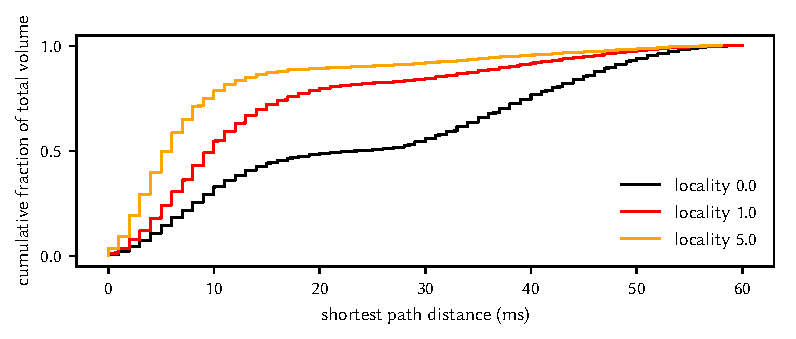
\includegraphics{tm_gen_cumulative_demands}
  \caption{Cumulative fraction of total volume in Cogent's topology
    that travels a given shortest-path distance.}
  \label{fig:tm-gen-cumulative}
\end{figure}

To see how the addition of locality in the second step behaves in
practice we examine three different traffic matrices generated with
the same seed and the same load value, but with three different values
of locality---0, 1 and 5. The topology is that of Cogent---the largest
one in the TopologyZoo~\cite{zoo} dataset, and one with high LLPD
(see~\cite{gvozdiev2018low}). In Figure~\ref{fig:tm-gen-cumulative} we
show the locality of traffic volume in each of the three traffic
matrices. To generate the plot we sort all aggregates based on the
length of their shortest path. Each point on the plot is a separate
traffic aggregate; the $x$ value is the length of the aggregate's
shortest path and the $y$ value is the cumulative fraction of the
total traffic volume in the entire traffic matrix.

Cogent's topology contains large European and North American parts,
connected by a handful of long-haul trans-oceanic links which account
for the flattening of the {\sc locality 0} curve. Looking at the that
curve, we can see that 50\% of the traffic volume travels 20 ms or
less---{\em i.e.,} about half of all traffic is between Europe and
North America. Recent studies of Deutsche Telekom's
network~\cite{schuller2017traffic} suggest that in large ISPs this is
not the case, but instead traffic is significantly more localized. As
we increase locality we notice that less and less traffic is being
moved between the two continents, loading the long-haul links less and
less. At the extreme of {\sc locality 5} only about 10\% of all
traffic crosses between Europe and North America, with long-haul links
being underutilized. We conjecture that this is also not a very
realistic scenario. {\sc locality 1}, which exhibits an 80/20 split
between local and remote traffic, is probably closer to reality.

\medskip
 
\bibliographystyle{unsrt}
\bibliography{biblio}

\end{document}
